\section{Problem Formulation and Benchmark}

\subsection{Defining One Tissue and Antigen-presenting Context (Tissue--MHC Task Definition)}

One task corresponds to one tissue and one \plainMHCI{} restriction. For example, lung with the human leukocyte antigen allele (HLA-A*02:01) and liver with the same human leukocyte antigen allele (HLA-A*02:01) are different tasks because the tissue context differs, even though the allele is the same. Let \(t\) denote a tissue and \(m\) a \plainMHCI{} restriction. We define the set of observed tasks as
\[
\mathcal{T}=\{\tau=(t,m)\}.
\]
Each benchmark row is represented by
\[
x_i=(p_i,\tau_i), \qquad y_i\in\{0,1\},
\]
where \(p_i\) is a nine-residue peptide and \(\tau_i\) is a task defined by one tissue and one antigen-presenting restriction (tissue--MHC task). A positive label, \(y_i=1\), indicates that the peptide has positive ligand evidence in the target tissue and antigen-presenting context (tissue--MHC context). A comparison label, \(y_i=0\), indicates that the peptide has positive evidence under the same antigen-presenting restriction (MHC restriction) and parent protein in at least one other tissue, but is not reported for the target tissue--antigen-presenting-molecule task (tissue--MHC task). Thus, a comparison peptide with evidence elsewhere but not in the target tissue (pseudo-negative) represents absence of recorded evidence rather than an experimentally verified non-presented peptide.

Given \((p,\tau)\), a model parameterized by \(\theta\) produces
\[
s_{\theta}(p,\tau)\in\mathbb{R},
\]
with larger values indicating stronger predicted evidence within tissue--antigen-presenting-molecule combination (task) \(\tau\). Operationally, the model learns to rank a peptide reported in the target tissue above the comparison peptide that shares its presenting restriction and parent protein (matched comparison peptide). It is trained on individual peptide rows, while the two-row construction (pair structure) controls example construction and evaluation. Because each tissue--antigen-presenting-molecule combination (tissue--MHC combination) has its own prediction function, the benchmark evaluates previously represented combinations; it does not assess unseen tissues or unseen antigen-presenting restrictions (MHC restrictions).

\subsection{Pairing Peptides That Share Tissue, Presenting Restriction, and Parent Protein (Matched-pair Design)}

Each pair \(j\) contains exactly one positive peptide \(p_j^{+}\) and one comparison peptide with evidence elsewhere but not in the target tissue (pseudo-negative peptide) \(p_j^{-}\). The two rows share the same target tissue, antigen-presenting restriction (MHC restriction), and parent UniProt protein:
\[
t_j^{+}=t_j^{-}, \qquad
m_j^{+}=m_j^{-}, \qquad
u_j^{+}=u_j^{-}.
\]
This matching removes two easy explanations for a difference: the peptides cannot be separated merely because they use different \plainMHC{} molecules or come from different proteins. The remaining difference can include tissue-associated processing and presentation, but also differences in cell composition, study design, detection sensitivity, and annotation completeness. The benchmark therefore measures tissue-associated evidence, not a purified molecular mechanism.

We first calculate performance separately for every tissue--antigen-presenting-molecule combination (tissue--MHC combination) and then give each task equal weight, so common tasks do not dominate rare ones. We also report the \plainPairAcc{}:
\[
\mathrm{WithinPairAccuracy\;(PairAcc)}
=
\frac{1}{N}
\sum_{j=1}^{N}
\mathbf{1}
\left[
s_{\theta}(p_j^{+},\tau_j)
>
s_{\theta}(p_j^{-},\tau_j)
\right],
\]
where \(N\) is the number of held-out pairs. The \plainPairAcc{} is the fraction of pairs for which the peptide reported in the target tissue receives the higher score. AUROC measures ordering across all rows within a task, whereas the \plainPairAcc{} directly evaluates concordance with the original comparison between peptides sharing presenting restriction and parent protein (matched biological comparison).

\subsection{Evidence Inclusion Criteria}

The human and mouse benchmarks are derived from the full ligand export of the \plainIEDB{} downloaded on July 4, 2026 \cite{vita2025iedb}. We apply the same biological inclusion rules to both species. We retain only clearly positive ligand records for \plainMHCI{} with an identifiable parent protein and a standard unmodified 9-amino-acid peptide:

\begin{itemize}
    \item a qualitative measurement whose normalized text begins with \emph{positive};
    \item a \plainMHCI{} restriction, with both peptide source and host matching Homo sapiens for the human benchmark or Mus musculus for the mouse benchmark;
    \item a human restriction matching the four-digit \plainHLA{} pattern \texttt{HLA-...*dd:dd} (the extractor also accepts the equivalent colon-free four-digit form) or a mouse restriction in the \plainHtwo{} beginning with \texttt{H2-};
    \item a parent UniProt accession extracted from the molecule-parent web identifier (internationalized resource identifier; IRI) in the \plainIEDB{};
    \item a linear, unmodified peptide containing only the 20 standard amino acids;
    \item a peptide length of exactly nine residues; and
    \item deduplication before pairing by the exact peptide, restriction, tissue, and parent/source-protein annotation fields.
\end{itemize}

Source-tissue values are stripped of surrounding whitespace and retained as the exact names used to define biological prediction combinations (task labels) in the \plainIEDB{}; distinct nonempty tissue strings are not merged after extraction. Empty or missing-value-like (\texttt{NA}-like) fields needed to define a biological prediction combination (task fields) are removed before benchmark filtering, which excludes 857 otherwise eligible human pairs, and pair-consistency checks require both rows to have the same nonempty tissue and restriction. Retained \plainHLA{} and \plainHtwo{} strings are used directly as identifiers for tissue--antigen-presenting-molecule combinations (task identifiers) after the pattern checks above. Records without a parent UniProt accession are excluded because parent-protein matching is a defining control of the benchmark. Restricting the study to unmodified canonical 9-residue peptides for \plainMHCI{} provides a consistent sequence space, but excludes variable-length ligands, post-translationally modified peptides, and presentation by class II antigen-presenting molecules (MHC-II).

\subsection{Constructing Peptide Pairs with the Same Restriction and Parent Protein (Matched-pair Construction)}

For each target tissue--antigen-presenting-molecule combination (tissue--MHC combination), we compare a peptide reported in that tissue with another peptide from the same protein that is reported in a different tissue under the same antigen-presenting restriction (MHC restriction). Pairs are generated with \plainSplitSeed{} 20260704 as follows:

\begin{enumerate}
    \item Group all eligible ligand records by antigen-presenting restriction (MHC restriction) \(m\) and parent UniProt protein \(u\).
    \item For each target combination \((t,m,u)\), collect peptides with positive evidence in tissue \(t\).
    \item From other tissues represented in the same \((m,u)\) group, collect candidate comparison peptides with evidence elsewhere but not yet in the target tissue (pseudo-negative peptides).
    \item Exclude every candidate that has any positive report in the target tissue--antigen-presenting-molecule task (tissue--MHC task) \((t,m)\).
    \item Within each target task and label, use each peptide at most once. For a given \((t,m,u)\) group, set the number of pairs to the smaller of the eligible positive and comparison-peptide (pseudo-negative) counts and sample both sets without replacement.
    \item Randomly permute the selected comparison peptides (pseudo-negatives) and join them one-to-one with the selected positives.
    \item Assign a persistent pair identifier, preserve the reported-tissue and protein annotations, and audit that every identifier has exactly one row per label, the same tissue, restriction, and parent UniProt in both rows (matched fields), and no comparison peptide (pseudo-negative) reported in the target tissue--antigen-presenting-molecule combination (target task).
\end{enumerate}

Every pair contributes one target-tissue peptide and one comparison peptide, so the dataset is deliberately balanced. This balance is useful for controlled ranking but does not resemble the natural frequency of presented peptides in a tissue sample. The reported scores therefore describe relative ranking within this constructed benchmark, not the probability that a peptide would be detected in a biological specimen.

\begin{figure}[tbp]
\centering
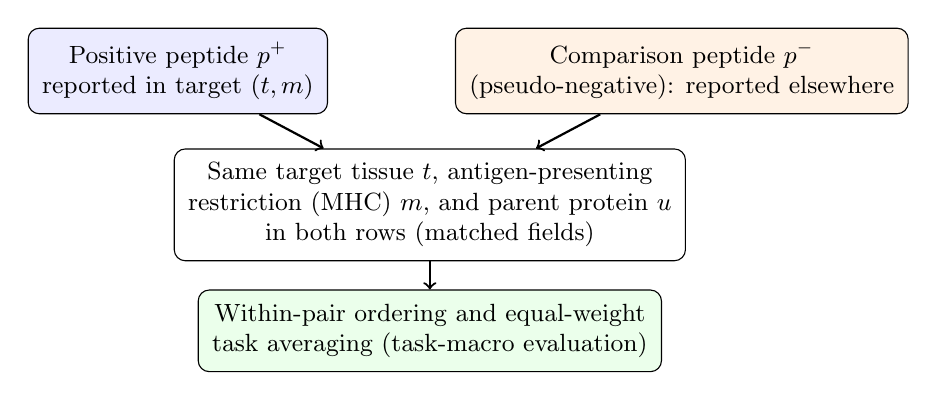
\begin{tikzpicture}[
    node distance=0.7cm,
    box/.style={draw,rounded corners,align=center,inner sep=5pt,font=\small},
    arr/.style={->,thick}
]
\node[box,fill=blue!8] (pos) at (-3.2,0) {Positive peptide \(p^{+}\)\\reported in target \((t,m)\)};
\node[box,fill=orange!10] (neg) at (3.2,0) {Comparison peptide \(p^{-}\)\\(pseudo-negative): reported elsewhere};
\node[box] (match) at (0,-1.7) {Same target tissue \(t\), antigen-presenting\\restriction (MHC) \(m\), and parent protein \(u\)\\in both rows (matched fields)};
\node[box,fill=green!8] (eval) at (0,-3.3) {Within-pair ordering and equal-weight\\task averaging (task-macro evaluation)};
\draw[arr] (pos) -- (match);
\draw[arr] (neg) -- (match);
\draw[arr] (match) -- (eval);
\end{tikzpicture}
\caption{Construction of two peptide rows sharing target tissue, antigen-presenting restriction, and parent protein (matched-pair construction). The comparison peptide has positive evidence elsewhere but no report in the target task (pseudo-negative).}
\label{fig:pair-construction}
\end{figure}

\subsection{Human Benchmark}

The current human and mouse benchmarks use the same rule for retaining a tissue--antigen-presenting-molecule combination (task-eligibility rule): a tissue--antigen-presenting-molecule task (tissue--MHC task) is retained only when it contains strictly more than 200 eligible peptide pairs sharing restriction and parent protein (matched pairs). Under this rule, the human benchmark contains 157 tissue--human-leukocyte-antigen tasks (tissue--HLA tasks); the smallest retained human task contains 201 pairs. Within each retained task, exactly 100 complete peptide pairs sharing restriction and parent protein (matched pairs) are sampled without replacement for the \plainFixedTest{}, and all remaining pairs form the training partition, using \plainSplitSeed{} 20260704. This saved internal train/test division (standard fixed split) contains the statistics summarized below.

\begin{table}[tbp]
\centering
\caption{Human benchmark statistics for the \plainFixedTest{}.}
\label{tab:human-benchmark-stats}
\small
\begin{tabular}{lr}
\toprule
Property & Value \\
\midrule
Tissue--human-leukocyte-antigen tasks (tissue--HLA tasks) & 157 \\
Tissues & 25 \\
\plainHLA{} alleles & 35 \\
Minimum eligible pairs per retained task & 201 \\
Training pairs & 73,798 \\
Test pairs & 15,700 \\
Training rows & 147,596 \\
Test rows & 31,400 \\
Test pairs per task & 100 \\
\bottomrule
\end{tabular}
\end{table}

The set of 157 tissue--\plainHLA{} combinations (157-task inventory) is summarized in Table~\ref{tab:human-benchmark-stats}. It forms an incomplete and long-tailed tissue-by-\plainHLA{} coverage matrix rather than a full set of all possible tissue--allele combinations (full Cartesian product). Calculating performance separately for each tissue--\plainHLA{} combination (task-wise evaluation) is therefore essential: a score calculated after pooling all rows (pooled metric) would overweight common tissue--\plainHLA{} combinations and could conceal weak performance on combinations with few examples (sparse tasks). The internal benchmark for already represented combinations (standard benchmark) holds out pair identifiers, but a peptide or parent protein may still occur in a different combination on both sides of the split. We accordingly treat it as an internal benchmark for familiar combinations (closed-task benchmark), rather than evidence that biological entities are completely new at evaluation (strict entity-level generalization).

For the \plainPeptideOOF{}, the complete 73,798-pair human training pool from the internal benchmark---excluding the separate 15,700-pair \plainFixedTest{}---is considered as a single pool. Pairs sharing either peptide are joined by following direct and indirect shared-peptide links (connected components) before fold assignment. This produces 17,036 connected groups (components), including 10,923 groups containing several pairs (multi-pair components); the largest group contains 755 pairs. A reproducible assignment that balances each task across folds (deterministic task-stratified assignment) distributes complete groups across three folds. Each held-out fold contains 24,598--24,600 pairs, each fitting set contains 49,198--49,200 pairs, all 157 tasks remain represented, and both complete-pair and exact-peptide overlap between fitting and held-out data are zero.

\subsection{Mouse Benchmark}

The mouse benchmark uses the same tissue-conditioned definition, in which the two peptides share their antigen-presenting restriction and parent protein (MHC- and parent-protein-matched task definition), and the same rule requiring more than 200 eligible pairs, using the \plainHtwo{} in place of \plainHLA{} alleles. This rule retains 24 tissue--mouse-antigen-presenting-system combinations (tissue--H2 tasks); the smallest retained combination (task) contains 224 pairs. Exactly 100 complete peptide pairs sharing target tissue, presenting restriction, and parent protein (matched pairs) per retained combination (task) are sampled without replacement for the \plainFixedTest{} with \plainSplitSeed{} 20260704, and the remainder form the training partition.

\begin{table}[tbp]
\centering
\caption{Mouse benchmark statistics for the \plainFixedTest{}.}
\label{tab:mouse-benchmark-stats}
\small
\begin{tabular}{lr}
\toprule
Property & Value \\
\midrule
Tissue--mouse-antigen-presenting-system tasks (tissue--H2 tasks) & 24 \\
Tissues & 13 \\
\plainHtwo{} restrictions & 4 \\
Minimum eligible pairs per retained task & 224 \\
Training pairs & 6,766 \\
\plainFixedTest{} pairs & 2,400 \\
Training rows & 13,532 \\
\plainFixedTest{} rows & 4,800 \\
\bottomrule
\end{tabular}
\end{table}

The mouse inventory is summarized in Table~\ref{tab:mouse-benchmark-stats}. The mouse \plainFixedTest{} is an internal partition that was \plainFrozen{}. The key boundary is the tissue--mouse-antigen-presenting-system task (tissue--H2 task): a held-out peptide is absent from the training rows of the task being evaluated, but it may occur in the training rows of another task. Table~\ref{tab:mouse-fixed-overlap} makes this distinction explicit. For every test row, the audit first asks whether its entity occurs in training for the same tissue--mouse-antigen-presenting-system task (tissue--H2 task); only if it does not, the audit asks whether it occurs in another task. The three columns are therefore mutually exclusive.

\begin{table}[tbp]
\centering
\caption{Mouse entity-overlap audit for the \plainFixedTest{}. Counts are test-row occurrences, except for pair identifiers, which are counted once per pair. ``Current task'' means the same tissue--mouse-antigen-presenting-system combination (tissue--H2 combination) as the test row.}
\label{tab:mouse-fixed-overlap}
\footnotesize
\setlength{\tabcolsep}{3pt}
\begin{tabular}{@{}>{\raggedright\arraybackslash}p{2.8cm}
                    >{\centering\arraybackslash}p{2.4cm}
                    >{\centering\arraybackslash}p{2.4cm}
                    >{\centering\arraybackslash}p{2.4cm}@{}}
\toprule
Held-out entity (counted unit) & Current-task training & Other-task training only & Absent from all training \\
\midrule
Pair identifier (2,400 pairs) & 0 (0\%) & 0 (0\%) & 2,400 (100\%) \\
Peptide identity (4,800 rows) & 0 (0\%) & 4,047 (84.31\%) & 753 (15.69\%) \\
Parent UniProt (4,800 rows) & 710 (14.79\%) & 3,756 (78.25\%) & 334 (6.96\%) \\
\bottomrule
\end{tabular}
\end{table}

Thus, the peptide in a test row is new to the specific tissue--mouse-antigen-presenting-system subproblem (tissue--H2 subtask) being evaluated, even though most such rows contain a peptide already observed while fitting a different subproblem (subtask). In unique-entity terms, 2,453 of 3,011 test peptides (81.47\%) and 967 of 1,088 parent proteins (88.88\%) occur somewhere in training. Parent proteins can also recur within the current tissue--mouse-antigen-presenting-system combination (current task) because several peptide pairs sharing restriction and parent protein (matched pairs) may come from the same protein. All 24 tissue--mouse-antigen-presenting-system combinations (tissue--H2 tasks) themselves are represented in training. The \plainFixedTest{} is therefore an internal confirmation in already represented combinations with peptide reuse across combinations (seen-task confirmation with cross-task peptide reuse); it is not an evaluation of peptides, proteins, or biological combinations (tasks) absent from all training, nor an independent external validation.

Mouse \plainPeptideOOF{} applies the same transitive grouping of pairs linked by shared peptides (connected-component construction) to all 6,766 training-pool pairs. Complete connected groups (components) are assigned to three folds while maintaining all 24 tasks in every held-out partition. Complete-pair and exact-peptide overlap are both zero; the largest connected group contains 50 pairs, and the number of held-out pairs per task ranges from 41 to 157, with 82--314 fitting pairs per task. These counts show that exact peptide separation across all tasks (global peptide separation) is feasible without deleting overlapping pairs after an initial random split.

\subsection{Evaluation Settings and Their Biological Meaning}

The terminology used during model development combines three different layers: how the data are divided, how repeated models are combined, and how saved predictions are compared. These layers do not define separate biological experiments. Table~\ref{tab:evaluation-protocols} gives a plain-language guide to the terms used in the code and result files. In particular, \plainOOF{} means that the available training pool is divided into several parts: each part is predicted once by a model fitted on the other parts. An \plainSeed{} identifies one run of the same model started from a different random state, and an average over several \plainSeeds{} combines their predictions. By contrast, a \plainSplitSeed{} reproduces random pair sampling or fold assignment and does not denote another trained model. A model that was \plainFrozen{} had its structure, tuning choices, random initializations, and combination rule decided before the relevant evaluation results were inspected.

\begin{table}[tbp]
\centering
\caption{Plain-language guide to evaluation terms used in this study. A data setting changes which observations are available for model fitting and evaluation. A model descriptor changes how models are trained or combined without defining a new data split. An analysis descriptor refers only to a comparison of saved predictions.}
\label{tab:evaluation-protocols}
\scriptsize
\setlength{\tabcolsep}{2pt}
\begin{tabular}{@{}>{\raggedright\arraybackslash}p{2.55cm}
                    >{\raggedright\arraybackslash}p{1.45cm}
                    >{\raggedright\arraybackslash}p{4.05cm}
                    >{\raggedright\arraybackslash}p{3.35cm}@{}}
\toprule
Term used in the project & Layer & What is done & Purpose and relationship to other terms \\
\midrule
\plainFixedTest{}
& Data setting
& For each tissue--antigen-presenting-molecule task (tissue--MHC task), 100 complete positive--constructed-negative pairs (positive--pseudo-negative pairs) are kept outside the training file. A model fitted on all remaining rows scores this saved set once.
& Main internal benchmark for familiar tasks. It contains different rows from either \plainOOF{} analysis and is not an external cohort. \\
\addlinespace
\plainPairOOF{}
& Data setting
& The training pool is divided into three folds within each task. Both rows from one pair always remain together; each row is predicted by a model fitted on the other two folds.
& Cross-validation used for model development and internal checking. The same peptide may still occur in the fitting rows of another task. \\
\addlinespace
Same-pool ordinary cross-validation averaged over three or five random initializations (matched standard three-/five-seed OOF)
& Comparison label
& \plainPairOOF{} is applied to exactly the same training-pool rows later used by \plainPeptideOOF{}. Human results average three \plainSeeds{} and mouse results average five \plainSeeds{}.
& Ordinary reference for the peptide-separated analysis. Both \plainOOF{} analyses ultimately score the same rows, but their fold memberships are not identical or pair-by-pair matched. \\
\addlinespace
Previously specified repeated-model evaluation on the saved internal test set (frozen multi-seed fixed test)
& Model descriptor plus saved test
& A previously chosen model is refitted on the full training file for each prespecified \plainSeed{}; predictions are then averaged on the \plainFixedTest{}. The mouse main result uses five \plainSeeds{}.
& \plainFrozen{} and averaging five \plainSeeds{} describe the model evaluation, not a new type of data split. \\
\addlinespace
\plainPeptideOOF{}
& Data setting
& Pairs linked by any shared peptide sequence are placed in the same fold. A held-out peptide sequence is therefore absent from the fitting rows of every task.
& Robustness test for new exact peptide identities in familiar tissue--antigen-presenting-molecule tasks (tissue--MHC tasks). It does not require held-out tissues, antigen-presenting-molecule alleles (MHC alleles), or parent proteins to be new. \\
\addlinespace
Peptide-separated cross-validation averaged over three or five random initializations (peptide-disjoint three-/five-seed OOF)
& Model descriptor plus \plainPeptideOOF{}
& The same peptide-separated folds are used for every \plainSeed{}, and the held-out predictions are averaged across \plainSeeds{}.
& Repeated-model implementation of the preceding data setting; it is not an additional split. \\
\addlinespace
\plainConnectedSplit{}
& Split algorithm
& Shared-peptide links are followed transitively: if pair A shares a peptide with B and B shares one with C, all three enter the same fold.
& The algorithm that enforces exact-peptide separation across all tasks. \plainConnectedSplit{} is not a separate biological setting. \\
\addlinespace
Within-task comparison of ordinary and peptide-separated results (paired task-level standard-versus-strict statistics)
& Statistical analysis
& For each tissue--antigen-presenting-molecule combination (task), a metric from \plainMatchedOOF{} is compared with the corresponding metric from \plainPeptideOOF{}; differences calculated for individual combinations (task-level differences) are then summarized.
& Quantifies how sensitive performance is to the change in fold construction. Exact-peptide separation (called ``strict'' in project files) is not fully independent validation. \\
\bottomrule
\end{tabular}
\end{table}

\paragraph{What is actually predicted.}
The benchmark is constructed from \plainMatchedPairs{}, but the main neural models do not receive a pair as a two-peptide input. They score one peptide row at a time using the peptide sequence and the identity of the tissue--antigen-presenting-molecule task (tissue--MHC task). The pair identifier is used to construct balanced recorded-positive and constructed-negative examples (positive and pseudo-negative examples) and to keep the two rows from the same \plainMatchedPair{} together during splitting. Training uses a separate present/absent loss for each row (row-level binary loss), and the primary AUROC and AUPRC values compare all recorded-positive and constructed-negative rows within a task. \plainPairAcc{}, reported separately, directly asks whether the recorded-positive member of each original pair receives the higher score. Thus, keeping both members of a pair in the same fold (pair grouping) protects data integrity during splitting; it does not mean that the main network is trained by directly comparing two peptides (a pairwise ranking loss).

\paragraph{Saved internal test set (\emph{standard fixed test}).}
For each task, the dataset builder randomly selects 100 complete pairs for the test file and assigns the remaining pairs to the training file. Because a peptide is used at most once within a task during pair construction, a test peptide is absent from the training rows of that same task. However, the same sequence may have been observed in another tissue--antigen-presenting-molecule task (tissue--MHC task) and can therefore contribute to shared model parameters. The \plainFixedTest{} consequently measures internal discrimination in already represented biological contexts, with cross-task information sharing allowed. The word \plainFrozen{} describes a partition or analysis choices saved before evaluation; it does not by itself mean that the test has never influenced the wider research process. The human \plainFixedTest{} was examined repeatedly during long-term model development, whereas the mouse \plainFixedTest{} was opened only after the model and its averaging over five \plainSeeds{} had been \plainFrozen{}.

\paragraph{Cross-validation that keeps both rows of every pair together (\emph{pair-grouped OOF}).}
\plainPairOOF{} uses only the training file. Within each task, complete pairs are randomly distributed across three folds with nearly equal sizes. Two folds fit the model and the third is held out; rotating this role gives one prediction for every row in the training pool. This design prevents the model that predicts a row from fitting either member of its pair. It also prevents exact peptide reuse within the current task because of the one-use-per-task construction rule. It does not prevent that peptide from appearing in a different fitting task. \plainPairOOF{} is therefore a development-stage estimate for familiar tasks, not an independent validation dataset. It also differs from the \plainFixedTest{} in evaluated rows and fitting-set size, so their numerical difference is descriptive rather than an effect attributable to one design choice.

\paragraph{Ordinary comparison on the same rows (\emph{matched standard OOF}).}
\plainMatchedOOF{} means that \plainPairOOF{} is applied to the exact training-pool rows used in \plainPeptideOOF{}. The two analyses use the same model family, set of \plainSeeds{}, number of folds, and pooled evaluation rows. Their numbers of examples for each tissue--antigen-presenting-molecule combination and fold (task-by-fold sizes) are also close. The ordinary folds are nevertheless generated independently within each tissue--antigen-presenting-molecule combination (task); they are not reconstructed to place the same pairs, proteins, or peptide-linked groups in corresponding folds. The comparison is useful because every metric calculated separately for one biological combination (task-level metric) uses the same collection of labeled rows. It should be interpreted as the observed sensitivity to two different training-data partitions, rather than as a perfectly isolated causal estimate of the contribution of repeated peptide identities.

\paragraph{Cross-validation that excludes every held-out peptide from all training tasks (\emph{global peptide-disjoint OOF}).}
To remove exact peptide reuse across tasks, each pair is treated as one point in a network (a graph node). Two pair points are linked if either member has the same peptide sequence. All pairs linked directly or through intermediate pairs form one connected group (a connected component), and the complete group is assigned to one fold. Consequently, neither member of a held-out pair, nor any exact copy of those peptide sequences in another task, can occur in the fitting rows. All tissue--antigen-presenting-molecule tasks (tissue--MHC tasks) remain represented during fitting, so \plainPeptideOOF{} asks a specific biological question: can the model recognize tissue-associated sequence preferences for peptide identities it has not previously seen, while operating in tissue and antigen-presenting-molecule contexts (MHC contexts) it already knows?

This construction changes more than the presence of an exact duplicate. A shared peptide can connect a chain of otherwise different pairs, causing the complete chain to move together. The resulting folds can also differ in parent-protein composition and in the distribution of related sequence patterns. Table~\ref{tab:oof-overlap-audit} illustrates this point: although parent protein is not an input to the main models and is not explicitly separated, its overlap decreases markedly when pairs connected by shared peptides are kept together (connected components). Accordingly, the difference between \plainMatchedOOF{} and \plainPeptideOOF{} is best described as the change in robustness after exact peptides are separated (peptide-separation robustness gap). It shows how much the reported performance changes under this stricter grouping rule, but it does not measure a pure or mechanism-specific contribution from repeated peptides (``peptide leakage contribution'').

\begin{table}[tbp]
\centering
\caption{Entity overlap in the same-pool held-out-fold cross-validation analyses (OOF analyses). Pair overlap is the number of complete pair identifiers shared between fitting and held-out rows. Peptide values give the fold range for the percentage of unique held-out peptide sequences also present in fitting. Protein values give the three-fold mean percentage of unique held-out parent proteins present in fitting.}
\label{tab:oof-overlap-audit}
\scriptsize
\setlength{\tabcolsep}{3pt}
\begin{tabular}{llrrr}
\toprule
Species & Cross-validation setting (OOF setting) & Pair overlap & Peptide seen in fitting & Protein seen in fitting \\
\midrule
Human & \plainMatchedOOF{} & 0 & 69.19--69.91\% & 90.64\% \\
Human & \plainPeptideOOF{} & 0 & 0\% & 65.26\% \\
Mouse & \plainMatchedOOF{} & 0 & 71.43--72.12\% & 80.69\% \\
Mouse & \plainPeptideOOF{} & 0 & 0\% & 14.37\% \\
\bottomrule
\end{tabular}
\end{table}

\paragraph{Prespecified models, cohort-relative score combination, and statistical comparison.}
For \plainPeptideOOF{}, the human and mouse model structures, training budgets, sets of \plainSeeds{}, and prediction-averaging rules were \plainFrozen{} before the peptide-separated results were examined. This prevents direct tuning to those results. It does not make the experiment fully nested, because the selected model structures had previously been developed using \plainPairOOF{} predictions from the same training-pool rows. \plainPeptideOOF{} is therefore a robustness evaluation of a previously selected pipeline. In addition, the human model converts its two branch outputs to order positions among the peptides in each held-out task (within-cohort ranks) before averaging them. This transformation uses no held-out labels, but the final score is relative to the other peptides evaluated in that cohort rather than a stand-alone calibrated probability. The mouse model instead averages probabilities directly across \plainSeeds{}.

The statistics comparing the same biological combinations under both settings (within-task paired statistics) are performed after prediction and do not create another split. They compare \plainMatchedOOF{} and \plainPeptideOOF{} separately for each tissue--antigen-presenting-molecule combination (task by task) because both cover the same pooled evaluation rows. Comparing corresponding combinations reduces variation caused by evaluating different sets of tissue--antigen-presenting-molecule combinations (task inventories), but it does not remove variation caused by different fold membership, groups of transitively linked peptide pairs (connected-component structure), or the resulting fitting-data composition.

\paragraph{Scope of the biological conclusion.}
Evaluation on familiar tasks with cross-task information sharing (standard evaluation) asks whether peptide sequence helps distinguish recorded positives from constructed negatives sharing presenting restriction and parent protein (matched pseudo-negatives) in familiar tissue--antigen-presenting-molecule contexts (tissue--MHC contexts). \plainPeptideOOF{} asks whether a substantial part of that signal remains when the exact held-out peptide sequences are removed from all fitting tasks. Neither setting demonstrates that a constructed negative (pseudo-negative) is biologically never presented, identifies a causal antigen-processing mechanism, or evaluates a new tissue, a new antigen-presenting-molecule allele (MHC allele), a new tissue--antigen-presenting-molecule combination (tissue--MHC combination), a new parent protein, a new study, or an external cohort. Parent proteins, studies, experimental platforms, and related peptide motifs may still recur. These boundaries define \plainPeptideOOF{} as an internal robustness analysis rather than fully independent biological validation.
